\documentclass[12pt]{article}
\usepackage[margin=1in]{geometry}
\usepackage{amsmath,amssymb,mathtools}
\usepackage{enumitem}
\usepackage{bm}
\usepackage{hyperref}
\usepackage{fancyhdr}
\usepackage{draftwatermark}
\usepackage{xcolor}
\usepackage{pgfplots}
\usepackage{titlesec}
\pgfplotsset{compat=newest}

%------------- TITLE AND METADATA -------------
\newcommand{\CourseCode}{HE2002 }
\newcommand{\CourseName}{Macroeconomics II}
\newcommand{\DocType}{Tutorial 10}

\title{
\CourseCode \CourseName \\[0.3em]
\large \DocType
}
\author{
  Academic Year 2025/2026, Semester 2 \\[0.25em]
  \textit{Quantitative Research Society @NTU}
}
\date{\today}

%------------- HEADER & FOOTER (for page 2 onward) -------------
\fancypagestyle{main}{
  \fancyhf{}
  \fancyhead[L]{\CourseCode \CourseName \ --\ \DocType}
  \fancyhead[R]{\href{https://qrsntu.org}{QRS@NTU}}
  \fancyfoot[C]{\thepage}
  \renewcommand{\headrulewidth}{0.4pt}
  \renewcommand{\footrulewidth}{0pt}
}

%------------- SIMPLE FOOTER (page 1 only) -------------
\fancypagestyle{plainfirst}{
  \fancyhf{}
  \renewcommand{\headrulewidth}{0pt}
  \renewcommand{\footrulewidth}{0pt}
  \fancyfoot[C]{\scriptsize\textcolor{gray}{\textit{For academic reference only. This document is provided for educational purposes and does not constitute an official question paper, answer key, or any formally authorised academic material. Its content is not guaranteed to be complete or accurate.}}}
}

%------------- WATERMARK -------------
\SetWatermarkText{Unofficial — QRS@NTU — qrsntu.org}
\SetWatermarkScale{1}
\SetWatermarkLightness{0.99}

%------------- SHORTCUTS -------------
\newcommand{\R}{\mathbb{R}}
\newcommand{\Rp}{\mathbb{R}_+}
\newcommand{\E}{\mathbb{E}}
\newcommand{\Var}{\mathrm{Var}}
\newcommand{\dotp}{\cdot}

%------------- STYLE -------------
\setlist[enumerate]{itemsep=0.32em, topsep=0.32em}
\setlist[itemize]{itemsep=0.22em, topsep=0.22em}

\titleformat{\subsubsection}[block]
{\normalfont\large\bfseries}
{}
{0pt}
{}

\titleformat{\paragraph}[block]
{\normalfont\normalsize\bfseries}
{}
{0pt}
{}

\titlespacing*{\paragraph}
{0pt}
{1.2ex}
{0.6ex}

\setcounter{secnumdepth}{0}
\setcounter{tocdepth}{4}

\begin{document}

\maketitle
\thispagestyle{plainfirst}
\pagestyle{main}
\bigskip

%====================================================
% OVERVIEW
%====================================================
\begin{center}
  \rule{0.8\textwidth}{0.4pt}\\[4pt]
  \textbf{Overview}\\[2pt]
  \rule{0.8\textwidth}{0.4pt}
\end{center}

\noindent
This tutorial covers:
\begin{itemize}[leftmargin=*]
  \item the Cobb--Douglas production function in per-worker form;
  \item steady-state capital per worker and output per worker in the Solow model;
  \item comparative statics for changes in the saving rate and the depreciation rate;
  \item transition dynamics following permanent parameter changes;
  \item how the ratio \(s/\delta\) governs the long-run position of the economy in simple growth models.
\end{itemize}

\bigskip

\newpage
\tableofcontents

\newpage
%====================================================
% QUESTION 1
%====================================================
\section{Question 1: The Cobb--Douglas Production Function and the Steady State}

\noindent
Chapter 11, Q7. The Cobb-Douglas production function.

\subsection{Problem}
Suppose that the economy’s production function is given by
\[
Y = K^\alpha N^{1-\alpha}
\]
and assume that \(\alpha = 1/3\)

\begin{enumerate}[label=(\alph*)]
    \item For a given saving rate, \(s\), and depreciation rate, \(\delta\), give an expression for capital per worker in the steady state.
    \item Give an expression for output per worker in the steady state.
    \item Solve for the steady-state level of output per worker when \(s = 0.32\) and \(\delta = 0.08\).
    \item Suppose that the depreciation rate remains constant at \(\delta = 0.08\), while the saving rate is reduced by half, to \(s = 0.16\). What is the new steady-state output per worker?
\end{enumerate}

\subsection{Solution}

\subsubsection{Method 1: Direct steady-state calculation from the Solow equation}
Let
\[
k:=\frac{K}{N},
\qquad
y:=\frac{Y}{N}.
\]
Since \(\alpha=1/3\), the production function becomes
\[
Y=K^{1/3}N^{2/3}.
\]
Dividing by \(N\),
\[
y=\frac{Y}{N}=\frac{K^{1/3}N^{2/3}}{N}=K^{1/3}N^{-1/3}=\left(\frac{K}{N}\right)^{1/3}=k^{1/3}.
\]
Hence the per-worker production function is
\[
y=f(k)=k^{1/3}.
\]

In the Solow model with no population growth and no technological progress, the law of motion for capital per worker is
\[
k_{t+1}-k_t=s f(k_t)-\delta k_t.
\]
At the steady state,
\[
k_{t+1}=k_t=k^*,
\]
so
\[
s f(k^*)=\delta k^*.
\]
Substituting \(f(k)=k^{1/3}\),
\[
s(k^*)^{1/3}=\delta k^*.
\]

\begin{enumerate}[label=(\alph*)]
    \item
    Solve
    \[
    s(k^*)^{1/3}=\delta k^*.
    \]
    For the positive steady state,
    \[
    s=\delta (k^*)^{2/3},
    \]
    so
    \[
    (k^*)^{2/3}=\frac{s}{\delta}.
    \]
    Raising both sides to the power \(3/2\),
    \[
    k^*=\left(\frac{s}{\delta}\right)^{3/2}.
    \]
    Therefore,
    \[
    \boxed{k^*=\left(\frac{s}{\delta}\right)^{3/2}.}
    \]

    \item
    The steady-state output per worker is
    \[
    y^*=f(k^*)=(k^*)^{1/3}.
    \]
    Using part (a),
    \[
    y^*=\left[\left(\frac{s}{\delta}\right)^{3/2}\right]^{1/3}
    =\left(\frac{s}{\delta}\right)^{1/2}.
    \]
    Hence
    \[
    \boxed{y^*=\left(\frac{s}{\delta}\right)^{1/2}.}
    \]

    \item
    If \(s=0.32\) and \(\delta=0.08\), then
    \[
    \frac{s}{\delta}=\frac{0.32}{0.08}=4.
    \]
    Therefore
    \[
    y^*=\left(\frac{s}{\delta}\right)^{1/2}=\sqrt{4}=2.
    \]
    So the steady-state level of output per worker is
    \[
    \boxed{y^*=2.}
    \]

    \item
    Now \(s=0.16\) and \(\delta=0.08\), so
    \[
    \frac{s}{\delta}=\frac{0.16}{0.08}=2.
    \]
    Hence the new steady-state output per worker is
    \[
    y^*=\sqrt{2}.
    \]
    Numerically,
    \[
    \sqrt{2}\approx 1.4142.
    \]
    Therefore,
    \[
    \boxed{y^*=\sqrt{2}\approx 1.4142.}
    \]
\end{enumerate}

\subsubsection{Method 2: Break-even investment and the ratio \(s/\delta\)}
Using
\[
y=k^{1/3},
\]
steady-state equilibrium is obtained where actual investment per worker equals break-even investment:
\[
s y=\delta k.
\]
Substituting \(y=k^{1/3}\),
\[
s k^{1/3}=\delta k.
\]
Divide both sides by \(k^{1/3}\) for the positive steady state:
\[
s=\delta k^{2/3}.
\]
So
\[
k^{2/3}=\frac{s}{\delta},
\qquad
k^*=\left(\frac{s}{\delta}\right)^{3/2}.
\]
Then
\[
y^*=(k^*)^{1/3}=\left(\frac{s}{\delta}\right)^{1/2}.
\]

\begin{enumerate}[label=(\alph*)]
    \item
    The positive steady-state capital per worker is
    \[
    \boxed{k^*=\left(\frac{s}{\delta}\right)^{3/2}.}
    \]

    \item
    The corresponding steady-state output per worker is
    \[
    \boxed{y^*=\left(\frac{s}{\delta}\right)^{1/2}.}
    \]

    \item
    When
    \[
    \frac{s}{\delta}=4,
    \]
    we get
    \[
    y^*=\sqrt{4}=2.
    \]
    Therefore,
    \[
    \boxed{y^*=2.}
    \]

    \item
    Halving the saving rate from \(0.32\) to \(0.16\) halves the ratio \(s/\delta\) from \(4\) to \(2\). Since steady-state output per worker depends on the square root of this ratio,
    \[
    y^*=\sqrt{\frac{s}{\delta}}=\sqrt{2}.
    \]
    Hence
    \[
    \boxed{y^*=\sqrt{2}\approx 1.4142.}
    \]
\end{enumerate}

\begin{center}
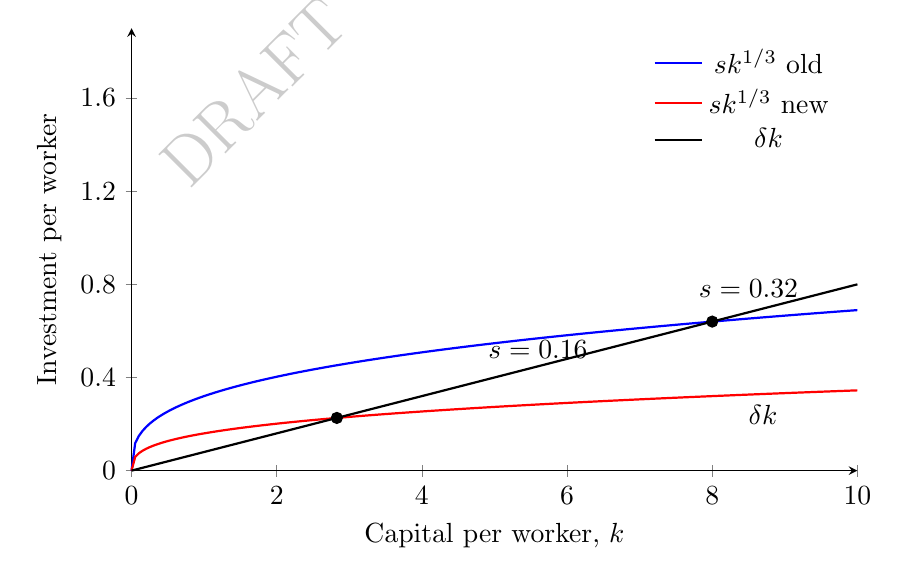
\begin{tikzpicture}
\begin{axis}[
    width=10.8cm,
    height=7.2cm,
    xmin=0,xmax=10,
    ymin=0,ymax=1.9,
    axis lines=left,
    xlabel={Capital per worker, \(k\)},
    ylabel={Investment per worker},
    xtick={0,2,4,6,8,10},
    ytick={0,0.4,0.8,1.2,1.6},
    legend style={draw=none, at={(0.98,0.98)}, anchor=north east},
    clip=false
]
\addplot[domain=0:10,samples=200,thick,blue] {0.32*x^(1/3)};
\addplot[domain=0:10,samples=200,thick,red] {0.16*x^(1/3)};
\addplot[domain=0:10,samples=2,thick,black] {0.08*x};
\addplot[only marks,mark=*,mark size=2pt] coordinates {(8,0.64) (2.828427,0.226274)};
\node at (axis cs:8.5,0.78) {\(s=0.32\)};
\node at (axis cs:5.6,0.52) {\(s=0.16\)};
\node at (axis cs:8.7,0.24) {\(\delta k\)};
\legend{\(s k^{1/3}\) old,\(s k^{1/3}\) new,\(\delta k\)}
\end{axis}
\end{tikzpicture}
\end{center}

\newpage
%====================================================
% QUESTION 2
%====================================================
\section{Question 2: A Permanent Rise in Depreciation}

\noindent
Chapter 11, Q8

\subsection{Problem}
Continuing with the logic from C11 Q7, suppose that the economy’s production function is given by
\[
Y = K^{1/3}N^{2/3}
\]
and that the saving rate, \(s\), and the depreciation rate, \(\delta\) are equal to \(0.10\).

\begin{enumerate}[label=(\alph*)]
    \item What is the steady-state level of capital per worker?
    \item What is the steady-state level of output per worker?
\end{enumerate}

Suppose that the economy is in steady state and that, in period \(t\), the depreciation rate increases permanently from \(0.10\) to \(0.20\).

\begin{enumerate}[label=(\alph*),start=3]
    \item What will be the new steady-state levels of capital per worker and output per worker?
    \item Compute the path of capital per worker and output per worker over the first three periods after the change in the depreciation rate.
\end{enumerate}

\subsection{Solution}

\subsubsection{Method 1: Per-worker law of motion and direct iteration}
The per-worker production function is
\[
y=f(k)=k^{1/3}.
\]
With no population growth and no technological progress, the law of motion is
\[
k_{t+1}=s f(k_t)+(1-\delta)k_t.
\]

\begin{enumerate}[label=(\alph*)]
    \item
    Initially \(s=\delta=0.10\). At the steady state,
    \[
    s k^{1/3}=\delta k.
    \]
    Hence
    \[
    0.10\,k^{1/3}=0.10\,k.
    \]
    For the positive steady state,
    \[
    k^{1/3}=k.
    \]
    Dividing by \(k^{1/3}\),
    \[
    k^{2/3}=1,
    \]
    so
    \[
    k^*=1.
    \]
    Therefore,
    \[
    \boxed{k^*=1.}
    \]

    \item
    Since
    \[
    y^*=(k^*)^{1/3},
    \]
    we get
    \[
    y^*=1^{1/3}=1.
    \]
    Hence
    \[
    \boxed{y^*=1.}
    \]

    \item
    After the permanent increase in depreciation, \(s=0.10\) and \(\delta=0.20\). The new steady state solves
    \[
    0.10\,k^{1/3}=0.20\,k.
    \]
    For the positive steady state,
    \[
    0.10=0.20\,k^{2/3},
    \]
    so
    \[
    k^{2/3}=\frac{0.10}{0.20}=\frac{1}{2}.
    \]
    Thus
    \[
    k^*=\left(\frac{1}{2}\right)^{3/2}=\frac{1}{2\sqrt{2}}=\frac{\sqrt{2}}{4}.
    \]
    The new steady-state output per worker is
    \[
    y^*=(k^*)^{1/3}=\left(\frac{1}{2}\right)^{1/2}=\frac{1}{\sqrt{2}}.
    \]
    Therefore,
    \[
    \boxed{k^*=\left(\frac{1}{2}\right)^{3/2}=\frac{1}{2\sqrt{2}}\approx 0.3536,}
    \]
    \[
    \boxed{y^*=\left(\frac{1}{2}\right)^{1/2}=\frac{1}{\sqrt{2}}\approx 0.7071.}
    \]

    \item
    The economy is initially at the old steady state, so
    \[
    k_t=1,
    \qquad
    y_t=1.
    \]
    After the shock, the new law of motion is
    \[
    k_{t+1}=0.10\,k_t^{1/3}+0.80\,k_t.
    \]

    \paragraph{Period \(t+1\).}
    \[
    k_{t+1}=0.10(1)^{1/3}+0.80(1)=0.10+0.80=0.90.
    \]
    Hence
    \[
    y_{t+1}=k_{t+1}^{1/3}=0.90^{1/3}\approx 0.9655.
    \]

    \paragraph{Period \(t+2\).}
    \[
    k_{t+2}=0.10\,k_{t+1}^{1/3}+0.80\,k_{t+1}
    =0.10(0.90^{1/3})+0.80(0.90).
    \]
    Numerically,
    \[
    k_{t+2}\approx 0.10(0.9655)+0.72\approx 0.8165.
    \]
    Therefore
    \[
    y_{t+2}=k_{t+2}^{1/3}\approx 0.8165^{1/3}\approx 0.9347.
    \]

    \paragraph{Period \(t+3\).}
    \[
    k_{t+3}=0.10\,k_{t+2}^{1/3}+0.80\,k_{t+2}
    \approx 0.10(0.9347)+0.80(0.8165)\approx 0.7467.
    \]
    Hence
    \[
    y_{t+3}=k_{t+3}^{1/3}\approx 0.7467^{1/3}\approx 0.9072.
    \]

    Thus the transition path is:
    \[
    \boxed{
    \begin{aligned}
    k_t&=1,      & y_t&=1,\\
    k_{t+1}&=0.9000, & y_{t+1}&\approx 0.9655,\\
    k_{t+2}&\approx 0.8165, & y_{t+2}&\approx 0.9347,\\
    k_{t+3}&\approx 0.7467, & y_{t+3}&\approx 0.9072.
    \end{aligned}}
    \]
\end{enumerate}

\subsubsection{Method 2: Break-even investment diagram and transition logic}
Before the shock, steady-state equilibrium is determined by the intersection of
\[
s f(k)=0.10\,k^{1/3}
\]
and
\[
\delta k=0.10\,k.
\]
After the shock, the saving curve is unchanged but the break-even line rotates upward to
\[
\delta k=0.20\,k.
\]

\begin{enumerate}[label=(\alph*)]
    \item
    The original steady state solves
    \[
    0.10\,k^{1/3}=0.10\,k.
    \]
    So
    \[
    \boxed{k^*=1.}
    \]

    \item
    Using \(y=k^{1/3}\),
    \[
    \boxed{y^*=1.}
    \]

    \item
    The new steady state solves
    \[
    0.10\,k^{1/3}=0.20\,k.
    \]
    Hence
    \[
    \boxed{k^*=\left(\frac{1}{2}\right)^{3/2}\approx 0.3536,}
    \qquad
    \boxed{y^*=\left(\frac{1}{2}\right)^{1/2}\approx 0.7071.}
    \]

    \item
    Since the economy starts at \(k_t=1\), which is above the new steady state \(0.3536\), depreciation now exceeds actual investment:
    \[
    0.20\,k_t > 0.10\,k_t^{1/3}.
    \]
    Therefore capital per worker must fall over time toward the new steady state. The first iterations are:
    \[
    k_{t+1}=0.10(1)^{1/3}+0.80(1)=0.90,
    \]
    \[
    k_{t+2}=0.10(0.90)^{1/3}+0.80(0.90)\approx 0.8165,
    \]
    \[
    k_{t+3}=0.10(0.8165)^{1/3}+0.80(0.8165)\approx 0.7467.
    \]
    Then
    \[
    y_{t+1}=0.90^{1/3}\approx 0.9655,
    \qquad
    y_{t+2}\approx 0.9347,
    \qquad
    y_{t+3}\approx 0.9072.
    \]
    Hence
    \[
    \boxed{
    \begin{aligned}
    k_{t+1}&=0.9000, & y_{t+1}&\approx 0.9655,\\
    k_{t+2}&\approx 0.8165, & y_{t+2}&\approx 0.9347,\\
    k_{t+3}&\approx 0.7467, & y_{t+3}&\approx 0.9072.
    \end{aligned}}
    \]
\end{enumerate}

\begin{center}
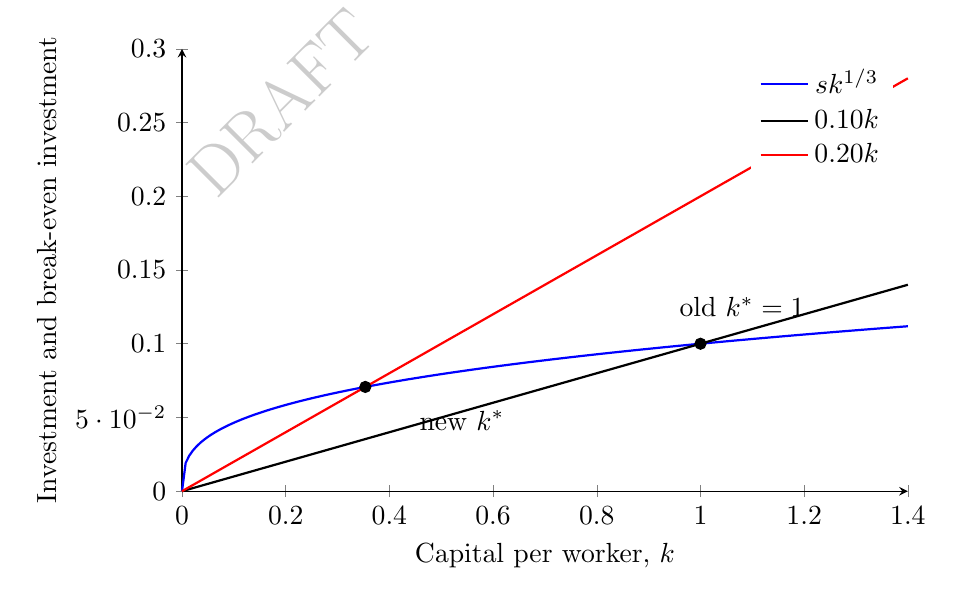
\begin{tikzpicture}
\begin{axis}[
    width=10.8cm,
    height=7.2cm,
    xmin=0,xmax=1.4,
    ymin=0,ymax=0.30,
    axis lines=left,
    xlabel={Capital per worker, \(k\)},
    ylabel={Investment and break-even investment},
    xtick={0,0.2,0.4,0.6,0.8,1.0,1.2,1.4},
    ytick={0,0.05,0.10,0.15,0.20,0.25,0.30},
    legend style={draw=none, at={(0.98,0.98)}, anchor=north east},
    clip=false
]
\addplot[domain=0:1.4,samples=200,thick,blue] {0.1*x^(1/3)};
\addplot[domain=0:1.4,samples=2,thick,black] {0.1*x};
\addplot[domain=0:1.4,samples=2,thick,red] {0.2*x};
\addplot[only marks,mark=*,mark size=2pt] coordinates {(1,0.1) (0.353553,0.070711)};
\node at (axis cs:1.08,0.125) {old \(k^*=1\)};
\node at (axis cs:0.54,0.048) {new \(k^*\)};
\legend{\(s k^{1/3}\),\(0.10k\),\(0.20k\)}
\end{axis}
\end{tikzpicture}
\end{center}

\newpage
%====================================================
% QUESTION 3
%====================================================
\section{Question 3: The Saving Rate and Changes in the Capital Stock}

\noindent
Chapter 11, Q9. The saving rate and changes in the capital stock

\subsection{Problem}
Assume the economy initially starts at its original steady state. Suppose that the economy’s production function is given by
\[
Y = \sqrt{K}\sqrt{N},
\]
and the saving rate, \(s\), slowly declines from 12\% in year \(t\) to 11\% in year \(t + 1\) and 10\% in year \(t + 2\). Suppose, moreover, that the depreciation rate, \(\delta\), is 10\%.

\begin{enumerate}[label=(\alph*)]
    \item what happens to the steady-state capital stock per worker and the steady-state output per worker? Please compute the actual values for capital stock per worker and output per worker from period \(t\) to \(t+3\).
    \item Assume that the depreciation rate increases to 12\% at time \(t\) (remaining stable afterwards). What is the new steady-state capital stock per worker the economy will approaches in the long run? What is the new steady-state output per worker? How does this compare to your answer to part a? Please compute the values for capital stock per worker and output per worker from period \(t\) to \(t+3\).
\end{enumerate}

\subsection{Solution}

\subsubsection{Method 1: Moving steady states and direct transition arithmetic}
Because
\[
Y=\sqrt{K}\sqrt{N},
\]
the per-worker production function is
\[
y=\frac{Y}{N}=\sqrt{\frac{K}{N}}=\sqrt{k}=k^{1/2}.
\]
The law of motion for capital per worker is
\[
k_{t+1}=s_t \sqrt{k_t} + (1-\delta_t)k_t.
\]
A steady state satisfies
\[
s\sqrt{k^*}=\delta k^*.
\]
For the positive steady state,
\[
s=\delta \sqrt{k^*},
\]
so
\[
\sqrt{k^*}=\frac{s}{\delta},
\qquad
k^*=\left(\frac{s}{\delta}\right)^2,
\qquad
y^*=\sqrt{k^*}=\frac{s}{\delta}.
\]

\begin{enumerate}[label=(\alph*)]
    \item
    Here \(\delta=0.10\) throughout, while
    \[
    s_t=0.12,\qquad s_{t+1}=0.11,\qquad s_{t+2}=0.10.
    \]
    Therefore the associated steady states are:
    \[
    \text{at }t:\quad
    k^*=\left(\frac{0.12}{0.10}\right)^2=1.44,
    \qquad
    y^*=\frac{0.12}{0.10}=1.20;
    \]
    \[
    \text{at }t+1:\quad
    k^*=\left(\frac{0.11}{0.10}\right)^2=1.21,
    \qquad
    y^*=\frac{0.11}{0.10}=1.10;
    \]
    \[
    \text{from }t+2\text{ onward}:\quad
    k^*=\left(\frac{0.10}{0.10}\right)^2=1,
    \qquad
    y^*=\frac{0.10}{0.10}=1.
    \]
    So both the steady-state capital stock per worker and the steady-state output per worker fall over time.

    Since the economy initially starts at its original steady state,
    \[
    k_t=1.44,
    \qquad
    y_t=\sqrt{1.44}=1.20.
    \]

    Because \(s_t=0.12\) in year \(t\),
    \[
    k_{t+1}=0.12(1.20)+0.90(1.44)=0.144+1.296=1.44.
    \]
    Hence
    \[
    y_{t+1}=\sqrt{1.44}=1.20.
    \]

    In year \(t+1\), the saving rate falls to \(0.11\), so
    \[
    k_{t+2}=0.11(1.20)+0.90(1.44)=0.132+1.296=1.428.
    \]
    Thus
    \[
    y_{t+2}=\sqrt{1.428}\approx 1.1950.
    \]

    In year \(t+2\), the saving rate falls to \(0.10\), so
    \[
    k_{t+3}=0.10\sqrt{1.428}+0.90(1.428).
    \]
    Using \(\sqrt{1.428}\approx 1.1950\),
    \[
    k_{t+3}\approx 0.10(1.1950)+1.2852=1.4047.
    \]
    Therefore
    \[
    y_{t+3}=\sqrt{1.4047}\approx 1.1852.
    \]

    Hence the actual path is
    \[
    \boxed{
    \begin{aligned}
    k_t&=1.4400, & y_t&=1.2000,\\
    k_{t+1}&=1.4400, & y_{t+1}&=1.2000,\\
    k_{t+2}&=1.4280, & y_{t+2}&\approx 1.1950,\\
    k_{t+3}&\approx 1.4047, & y_{t+3}&\approx 1.1852.
    \end{aligned}}
    \]

    \item
    Interpreting part (b) as a new scenario, keep the saving rate at its original level \(s=0.12\), and suppose the depreciation rate rises permanently from \(0.10\) to \(0.12\) at time \(t\).

    The new long-run steady state therefore satisfies
    \[
    k^*=\left(\frac{0.12}{0.12}\right)^2=1,
    \qquad
    y^*=\frac{0.12}{0.12}=1.
    \]
    So
    \[
    \boxed{k^*=1,\qquad y^*=1.}
    \]

    Compared with part (a), the long-run steady state is the same as the eventual one reached there:
    \[
    (k^*,y^*)=(1,1).
    \]
    The difference is the transition path. In part (b), the downward adjustment starts immediately at time \(t\) because the depreciation shock is immediate and permanent.

    Since the economy again starts from the original steady state,
    \[
    k_t=1.44,
    \qquad
    y_t=1.20.
    \]
    The new law of motion is now
    \[
    k_{t+1}=0.12\sqrt{k_t}+0.88k_t.
    \]

    Thus
    \[
    k_{t+1}=0.12(1.20)+0.88(1.44)=0.144+1.2672=1.4112,
    \]
    so
    \[
    y_{t+1}=\sqrt{1.4112}\approx 1.1879.
    \]

    Next,
    \[
    k_{t+2}=0.12\sqrt{1.4112}+0.88(1.4112).
    \]
    Using \(\sqrt{1.4112}\approx 1.1879\),
    \[
    k_{t+2}\approx 0.12(1.1879)+1.2419\approx 1.3844,
    \]
    and hence
    \[
    y_{t+2}=\sqrt{1.3844}\approx 1.1766.
    \]

    Finally,
    \[
    k_{t+3}=0.12\sqrt{1.3844}+0.88(1.3844).
    \]
    Using \(\sqrt{1.3844}\approx 1.1766\),
    \[
    k_{t+3}\approx 0.12(1.1766)+1.2183\approx 1.3595,
    \]
    so
    \[
    y_{t+3}=\sqrt{1.3595}\approx 1.1660.
    \]

    Therefore the path is
    \[
    \boxed{
    \begin{aligned}
    k_t&=1.4400, & y_t&=1.2000,\\
    k_{t+1}&=1.4112, & y_{t+1}&\approx 1.1879,\\
    k_{t+2}&\approx 1.3844, & y_{t+2}&\approx 1.1766,\\
    k_{t+3}&\approx 1.3595, & y_{t+3}&\approx 1.1660.
    \end{aligned}}
    \]
\end{enumerate}

\subsubsection{Method 2: The \(s/\delta\) ratio and comparison of transition paths}
For the production function
\[
y=\sqrt{k},
\]
steady-state equilibrium satisfies
\[
s\sqrt{k^*}=\delta k^*.
\]
Thus
\[
\sqrt{k^*}=\frac{s}{\delta},
\qquad
k^*=\left(\frac{s}{\delta}\right)^2,
\qquad
y^*=\frac{s}{\delta}.
\]
So both long-run capital per worker and long-run output per worker are determined entirely by the ratio \(s/\delta\).

\begin{enumerate}[label=(\alph*)]
    \item
    In part (a), the ratio \(s/\delta\) changes as follows:
    \[
    \frac{s_t}{\delta}=\frac{0.12}{0.10}=1.2,
    \qquad
    \frac{s_{t+1}}{\delta}=\frac{0.11}{0.10}=1.1,
    \qquad
    \frac{s_{t+2}}{\delta}=\frac{0.10}{0.10}=1.
    \]
    Therefore the corresponding steady states move from
    \[
    (k^*,y^*)=(1.44,1.20)
    \]
    to
    \[
    (1.21,1.10)
    \]
    and then to
    \[
    (1,1).
    \]
    The economy therefore converges toward progressively lower steady states.

    The actual path, using
    \[
    k_{t+1}=s_t\sqrt{k_t}+0.90k_t,
    \]
    is exactly the same as in Method 1:
    \[
    \boxed{
    \begin{aligned}
    k_t&=1.4400, & y_t&=1.2000,\\
    k_{t+1}&=1.4400, & y_{t+1}&=1.2000,\\
    k_{t+2}&=1.4280, & y_{t+2}&\approx 1.1950,\\
    k_{t+3}&\approx 1.4047, & y_{t+3}&\approx 1.1852.
    \end{aligned}}
    \]

    \item
    In part (b), with \(s=0.12\) fixed and \(\delta\) rising to \(0.12\), the ratio becomes
    \[
    \frac{s}{\delta}=\frac{0.12}{0.12}=1.
    \]
    So the new long-run steady state is immediately
    \[
    \boxed{(k^*,y^*)=(1,1).}
    \]
    This is the same long-run destination as in part (a), but reached under a different mechanism:
    \begin{itemize}[leftmargin=*]
        \item in part (a), the saving rate falls gradually, so the steady state shifts downward in stages;
        \item in part (b), the depreciation rate jumps immediately, so the economy begins declining right away.
    \end{itemize}

    The transition path is
    \[
    \boxed{
    \begin{aligned}
    k_t&=1.4400, & y_t&=1.2000,\\
    k_{t+1}&=1.4112, & y_{t+1}&\approx 1.1879,\\
    k_{t+2}&\approx 1.3844, & y_{t+2}&\approx 1.1766,\\
    k_{t+3}&\approx 1.3595, & y_{t+3}&\approx 1.1660.
    \end{aligned}}
    \]
    Relative to part (a), the decline begins earlier and is faster over the first few periods because the higher depreciation rate bites immediately.
\end{enumerate}

\begin{center}
\renewcommand{\arraystretch}{1.25}
\begin{tabular}{|c|c|c|c|c|}
\hline
Period & \multicolumn{2}{c|}{Part (a): falling \(s\)} & \multicolumn{2}{c|}{Part (b): higher \(\delta\)} \\
\cline{2-5}
& \(k_t\) & \(y_t\) & \(k_t\) & \(y_t\) \\
\hline
\(t\)   & 1.4400 & 1.2000 & 1.4400 & 1.2000 \\
\(t+1\) & 1.4400 & 1.2000 & 1.4112 & 1.1879 \\
\(t+2\) & 1.4280 & 1.1950 & 1.3844 & 1.1766 \\
\(t+3\) & 1.4047 & 1.1852 & 1.3595 & 1.1660 \\
\hline
\end{tabular}
\end{center}

\end{document}